\lhead{\begin{tikzpicture}[remember picture, overlay]
    \node [anchor=100,inner sep=0] (imagenIZQUIERDA) at (current page header area.north){
\includegraphics[width=18cm]{img/Encabezado.PNG}};
    \end{tikzpicture}}
    \rhead{Ángeles-Hurtado}
    \rfoot{\begin{tikzpicture}[remember picture, overlay]
    \node [anchor=140,inner sep=0] (imagenDERECHA) at (current page footer area.south){
\includegraphics[width=18cm]{img/Foot.PNG}};
    \end{tikzpicture}}
    %----------------------------------------------------------------------------------------
    \lfoot{ \thepage}
    % \renewcommand{\labelenumi}{\alph{enumi}.)} 
    %----------------------------------------------------------------------------------------
    %----------------------------------------------------------------------------------------
    %	TITLE SECTION
    %----------------------------------------------------------------------------------------
    
    \setlength{\droptitle}{-5\baselineskip} % Move the title up
    \title{\textbf{Estudio de tiempos y movimientos en el ensamble de un circuito electrónico utilizando diferentes métodos para su optimización }} % Article title
    
     \author{ 
     \textsc{González-Pájaro, Alexa Giovana}\\ 
    %  Afiliación:
     \texttt{ Instituto Tecnológico de Querétaro } \\ 
     \texttt{Tecnológico Nacional de México } \\ 
     \texttt{Querétaro, México}\\ 
     \texttt{gonzalexa076@gmail.com} 
     \and 
     \textsc{Ángeles-Hurtado, Luis Alberto}\\ 
    %  Afiliación:
     \texttt{ Instituto Tecnológico de Querétaro } \\ 
     \texttt{ Tecnológico Nacional de México } \\ 
     \texttt{Querétaro, México}\\ 
     \texttt{alb3rt0.ah@gmail.com} 
    }
    
    
    %----------------------------------------------------------------------------------------
    
    % \begin{document}
    
    % Print the title
    \maketitle
    \thispagestyle{fancy}
    
    %----------------------------------------------------------------------------------------
    %	ARTICLE CONTENTS
    %----------------------------------------------------------------------------------------
    
    % \section*{Resumen}
    % \textit{Palabras clave:}
    % El resumen (ancho de página) deberá contener entre 100 y 200 palabras tipo Adobe Devangari 11 puntos.
    
    \begin{abstract}
    \noindent 
    El resumen (ancho de página) deberá contener entre 100 y 200 palabras tipo Adobe Devangari 11 puntos.
    
    \end{abstract}
    % 
    % 
    \textbf{\textit{Palabras clave}}: {First keyword should be the corresponding to the research area according with the authors guide. Maximum of 6 keywords.}
    % \keywords{First keyword should be the corresponding to the research area according with the authors guide. Maximum of 6 keywords.}
    
    \section{Introducción}
    
    % Define estudio de tiempos y movimientos 
    % define que es ensamble
    % define que es circuito electronico
    % define el metodo de tiempos predeterminados
    % define optimización
    \begin{itemize}
        \item El estudio de tiempos y movimientos es como observar detalladamente cómo se hace algo en el trabajo. Por ejemplo, cuando se ensamblan cosas como circuitos electrónicos, se analiza cómo se hace cada paso para hacerlo más eficiente. Así, se establecen tiempos estándar para cada tarea, lo que ayuda a hacer el trabajo más rápido y mejor. En resumen, analizar cómo hacemos las cosas y mejorarlas nos ayuda a trabajar de manera más eficiente y producir productos de mejor calidad.
        \cite{estudio}
        \item Las metodologías más usadas son el MTM (Método de Tiempos Predeterminados) para establecer estándares de tiempo en tareas, y el Lean Manufacturing para optimizar procesos eliminando desperdicios.
        \cite{metodología}
        \item En los últimos años, ha habido un avance significativo en la integración de tecnologías digitales en el estudio de tiempos y movimientos. Esto incluye el uso de software especializado que permite una recopilación más precisa de datos, análisis más detallados y simulaciones virtuales de procesos. Además, la implementación de técnicas de inteligencia artificial y aprendizaje automático está contribuyendo a la automatización y optimización de tareas dentro de los procesos de trabajo, lo que lleva a una mayor eficiencia y productividad.
        \item  Nuestro principal objetivo es buscar aumentar la eficiencia, reducir costos, mejorar la calidad y garantizar la seguridad en el lugar de trabajo. 
      %  \item Debe de tener Referencias científicas, URL, tesis, etc.
    \end{itemize}
    % 
    % 
    \section{Justificación}
    
    \begin{itemize}
        \item En la actualidad, existe una demanda creciente de eficiencia y calidad en la industria electrónica a nivel global, los consumidores esperan productos de alta calidad que sean fabricados de manera rápida y eficiente. En este contexto, el estudio de tiempos y movimientos en el ensamble de circuitos electrónicos se vuelve fundamental, se requiere una comprensión detallada de cada paso del proceso de ensamble para identificar oportunidades de mejora y optimización.
    \cite{optimización}
    Las empresas buscan métodos y herramientas que les permitan optimizar sus procesos de producción para ser más competitivas en el mercado global. El uso de diferentes métodos de optimización, como el Lean Manufacturing, Six Sigma o la automatización, se vuelve esencial para alcanzar estos objetivos. Estos métodos permiten reducir costos, minimizar desperdicios y mejorar la calidad del producto final.
    
    A nivel local o nacional, las empresas enfrentan desafíos específicos relacionados con la competitividad, la mano de obra y la disponibilidad de recursos. El estudio de tiempos y movimientos en el ensamble de circuitos electrónicos les ofrece una oportunidad para mejorar su eficiencia operativa y mantenerse a la par con las normas internacionales de calidad y producción.
    
    Además, el desarrollo de capacidades locales en el ámbito del estudio de tiempos y movimientos puede fomentar la innovación y el crecimiento económico en el país. La formación de profesionales especializados en estas áreas contribuye a fortalecer la industria nacional y a generar empleo calificado.
        \item Debe de tener Referencias científicas, URL, tesis, etc.
    \end{itemize}
    % 
    % 
    \section{Descripción del problema}
    \begin{itemize}
        \item En la actualidad, el ensamblaje del circuito se enfrenta a problemas importantes relacionados con la eficiencia y la productividad. Frecuentemente, los trabajadores tienen que seguir instrucciones complicadas y poco claras, lo que resulta en problemas con la calidad del ensamblaje y en tiempos de ciclo más prolongados de lo necesario.
        \item Una de las incógnitas para los científicos es cómo hacer que el proceso de ensamblaje sea mejor al dar a los trabajadores instrucciones simples y fáciles de entender. Esto podría hacer que el ensamblaje de circuitos electrónicos sea más eficiente y de mejor calidad.
        \item Debe de tener Referencias científicas, URL, tesis, etc.
    \end{itemize}
    \cite{ensamblaje}
    \textbf{*La incógnita científica es el elemento cuya solución incrementa el conocimiento científico.}
    % 
    % 
    \section{Fundamentación teórica}
    
    El estudio de tiempos y movimientos en el ensamble de circuitos electrónicos se basa en la búsqueda de la eficiencia, la optimización de procesos y la mejora continua para alcanzar los objetivos de calidad y competitividad en la industria electrónica.
    \begin{itemize}
        \item Si se lleva a cabo un análisis de tiempos y movimientos detallado en el proceso de ensamble de circuitos electrónicos, entonces se identificarán oportunidades para eliminar movimientos innecesarios y optimizar el flujo de trabajo, lo que conducirá a una mayor eficiencia y productividad.
        \item El principal objetivo es optimizar el proceso de producción para lograr una mayor eficiencia, calidad y competitividad en la industria electrónica.
        \item Las metodologías que se pueden utilizar para mejorar el ensamble de circuitos electrónicos son:
     Método de Tiempos Predeterminados: Establece tiempos estándar para cada tarea.
    Lean Manufacturing: Elimina desperdicios y optimiza el flujo de trabajo.
    Seis Sigma: Reduce errores y mejora continuamente el proceso.
    Simulación por Computadora: Modela el proceso para probar mejoras.
    Ergonomía: Diseña lugares de trabajo seguros y eficientes.
    Análisis de Datos: Identifica patrones y toma decisiones basadas en datos.
    
        \item Referencias solo de artículos y libros científicos.
    \end{itemize}
    % 
    % 
    \section{Hipótesis}
    
    Es la suposición con fundamento científico relativa a la solución del problema, necesidad o de cómo se aprovecha la oportunidad con la incógnita científica y se fundamenta con: 1. Una suposición (en afirmativo o negativo) y ésta deberá vincularse con:
    2. La fundamentación científica que deberá ser precisa 3. Una entidad de comparación para probar la suposición y
    4. La variable con que se califica o cuantifica la comparación o se prueba la hipótesis.
    
    \begin{itemize}
        \item Se debe de identificar claramente la suposición científica
        \item Se debe de identificar claramente el fundamento científico
        \item Se debe identificar claramente la variable de respuesta
        \item Se debe identifican claramente las realidades o modelos contrastantes
        \item Se debe de establecer las variables asociadas, explicativas o que tienen relación funcional con la variable de respuesta
    \end{itemize}
    % 
    % 
    \section{Objetivo}
    
    Precisar la acción necesaria para probar la hipótesis. Dicha acción se establece mediante el uso de verbos activos y en infinitivo.
    \begin{itemize}
        \item Se debe establecer que se pretende probar la hipótesis
    \end{itemize}
    
    \subsection{Objetivos específicos }
    
    \begin{itemize}
        \item Se debe establecer como un conjunto de acciones comunes para lograr el objetivo general
        \item Se debe establecer como etapas para lograr el objetivo general
    \end{itemize}
    
    Son actividades orientadas al cumplimiento del objetivo general. Se establecen con verbos activos en infinitivo. Son parte de la acción encaminada a probar la hipótesis. Éstos deben ser precisos, y en lo posible evitar aspectos metodológicos.
    % 
    % 
    \section{Cuerpo (Metodología, modelo matemático, etc.)}
    
    
    Cable de fibra óptica MH: Este tipo de cable se utiliza para transmitir señales de datos a través de fibras ópticas. Las especificaciones pueden incluir el tipo de fibra (monomodo o multimodo), el diámetro de la fibra, la capacidad de transmisión de datos (por ejemplo, 10 Gbps, 40 Gbps, etc.), la cubierta exterior (por ejemplo, PVC, LSZH), entre otros.
    \ref{anexo:cables}
    
     Cable de fibra óptica multimodo: Se utiliza para transmitir señales de datos a través de fibras ópticas que tienen un núcleo más grande que las fibras monomodo. Estas fibras permiten que múltiples modos de luz se propaguen a través del núcleo, lo que facilita la transmisión de datos a distancias más cortas y a velocidades más altas que los cables de fibra óptica monomodo. Los cables MM son comúnmente utilizados en aplicaciones de redes locales (LAN), enlaces de fibra corta y conexiones dentro de los centros de datos.
    \ref{anexo:cables}
    
    ESP32-C6: Es un microcontrolador de bajo consumo y alta eficiencia energética desarrollado por Espressif Systems. Es parte de la serie ESP32 de microcontroladores de bajo costo y alto rendimiento, que se utilizan ampliamente en una variedad de aplicaciones de IoT (Internet de las cosas), automatización del hogar, dispositivos conectados, y más.
    Características principales del ESP32-C6:
    1.	Procesador: Incorpora un procesador RISC de 32 bits de Espressif, con velocidades de reloj de hasta 160 MHz.
    2.	Conectividad: Ofrece conectividad Wi-Fi 802.11 b/g/n y BLE (Bluetooth Low Energy) para la comunicación inalámbrica.
    3.	Seguridad: Incluye características de seguridad avanzadas, como cifrado AES, generación de números aleatorios y certificados digitales, para proteger la integridad de los datos y las comunicaciones.
    4.	Bajo consumo de energía: Diseñado para minimizar el consumo de energía, lo que lo hace ideal para aplicaciones alimentadas por batería y dispositivos IoT de bajo consumo.
    5.	Interfaces de E/S: Ofrece una variedad de interfaces de E/S, incluyendo UART, SPI, I2C, ADC, DAC, PWM, y más, para facilitar la conexión y control de periféricos externos.
    6.	Memoria: Cuenta con memoria flash integrada para almacenamiento de programas y datos, así como RAM para ejecutar aplicaciones.
    7.	Soporte para desarrollo: Es compatible con el entorno de desarrollo integrado (IDE) de Arduino y el software de desarrollo ESP-IDF de Espressif, lo que facilita el desarrollo de aplicaciones y proyectos.
    \ref{anexo:ESP32-C6}
    
    LCD(Liquid Crystal Display): Es un tipo de pantalla que utiliza cristales líquidos para producir imágenes visibles. Está compuesto por una capa líquida colocada entre dos placas polarizadoras y electrodos transparentes. Los cristales líquidos pueden manipularse eléctricamente para controlar la cantidad de luz que pasa a través de ellos, lo que permite crear imágenes o texto en la pantalla.
    \ref{anexo:LCD 16x2}
    
    Potenciómetro:  Es un componente electrónico que se utiliza para variar la resistencia eléctrica de un circuito de manera manual. Consiste en un resistor con tres terminales: dos conexiones fijas (extremos) y una conexión deslizante (cursor). Al girar el eje del potenciómetro, el cursor se desplaza a lo largo del resistor, lo que cambia la resistencia eléctrica entre el terminal móvil y cada uno de los terminales fijos.
    
     Resistencia:Es un componente pasivo que se opone al flujo de corriente eléctrica en un circuito. Su función principal es limitar la corriente y reducir la cantidad de energía que fluye a través de ella. Las resistencias están diseñadas para tener un valor específico de resistencia eléctrica, medida, que determina la cantidad de oposición que ofrecen al flujo de corriente.
    \ref{anexo:resistencia}
    
    
    \begin{itemize}
        \item Se debe establecer que se habrá de hacer, como, conque, y donde para obtener la información que permita probar la hipótesis.  
        \item Se debe desglosar de acuerdo a los objetivos específicos. 
        \item Se debe establecer una estrategia metodológica por cada objetivo específico. De manera simplista se podría decir que se cambia el verbo en infinitivo por su respectivo adverbio.
        \item En cada objetivo se debe describir que método, que materiales y que equipo se usará para conseguirlo.
       % \item Se deben tener referencias Figura \ref{fig:lcd-16x2}.
    \end{itemize}
    Para acceder al manual sobre el ensamble ir a la siguiente referencia
    Manual \ref{anexo:Instructivo}
    % 
    % 
    
    % 
    % 
    \subsection{Prepara tu documento}
    
    Antes de que comiences a utilizar esta plantilla, es recomendable que prepare la información que contendrá en un archivo aparte. 
    Ten preparadas tus gráficas, así como también las tablas aparte, para que sea más fácil integrarlo. 
    Se recomienda fuertemente el uso de \textbf{formato Enhanced Metafile (.emf) para imágenes y gráficas} de resolución óptima. 
    Finalmente, completa y organiza el contenido antes de darle el formato de esta plantilla. 
    
    \subsection{Acrónimos y Abreviaciones}
    
    Los acrónimos y abreviaciones deberán ser definidos únicamente la primera vez que aparecen en el texto, esto para que el lector entienda lo que significan.
    
    \subsection{Ecuaciones}
    
    Las ecuaciones son una excepción a las especificaciones prescritas de esta plantilla. 
    Deberá determinar si su ecuación debe escribirse o no utilizando la fuente Adobe Devangari. 
    Para crear ecuaciones multinivel, puede ser necesario tratar la ecuación como un gráfico e insertarla en el texto después de aplicar el estilo de la platilla.
    Las ecuaciones serán enumeradas de manera consecutiva, y el número de ecuación, entre paréntesis, se colocan al ras de la derecha, utilizando una tabulación derecha. 
    
    \begin{equation}
        \label{eq1}
        x + y = z 
    \end{equation}
    
    Es importante asegurarse de que los símbolos de la ecuación sean definidos antes o inmediatamente después de la ecuación. Utilice “(1)”, en vez de “Eq. 1” al enumerar las ecuaciones, excepto al principio de una oración: “La ecuación (\ref{eq1}) es…”
    
    \section{Resultados y discusión}
    
    Estos son los resultados obtenidos mediante el uso del Instructivo
    \newpage
    %
    \centering{\section[\appendixautorefname{}]{Apéndice}}\label{anexo:evidencias}
    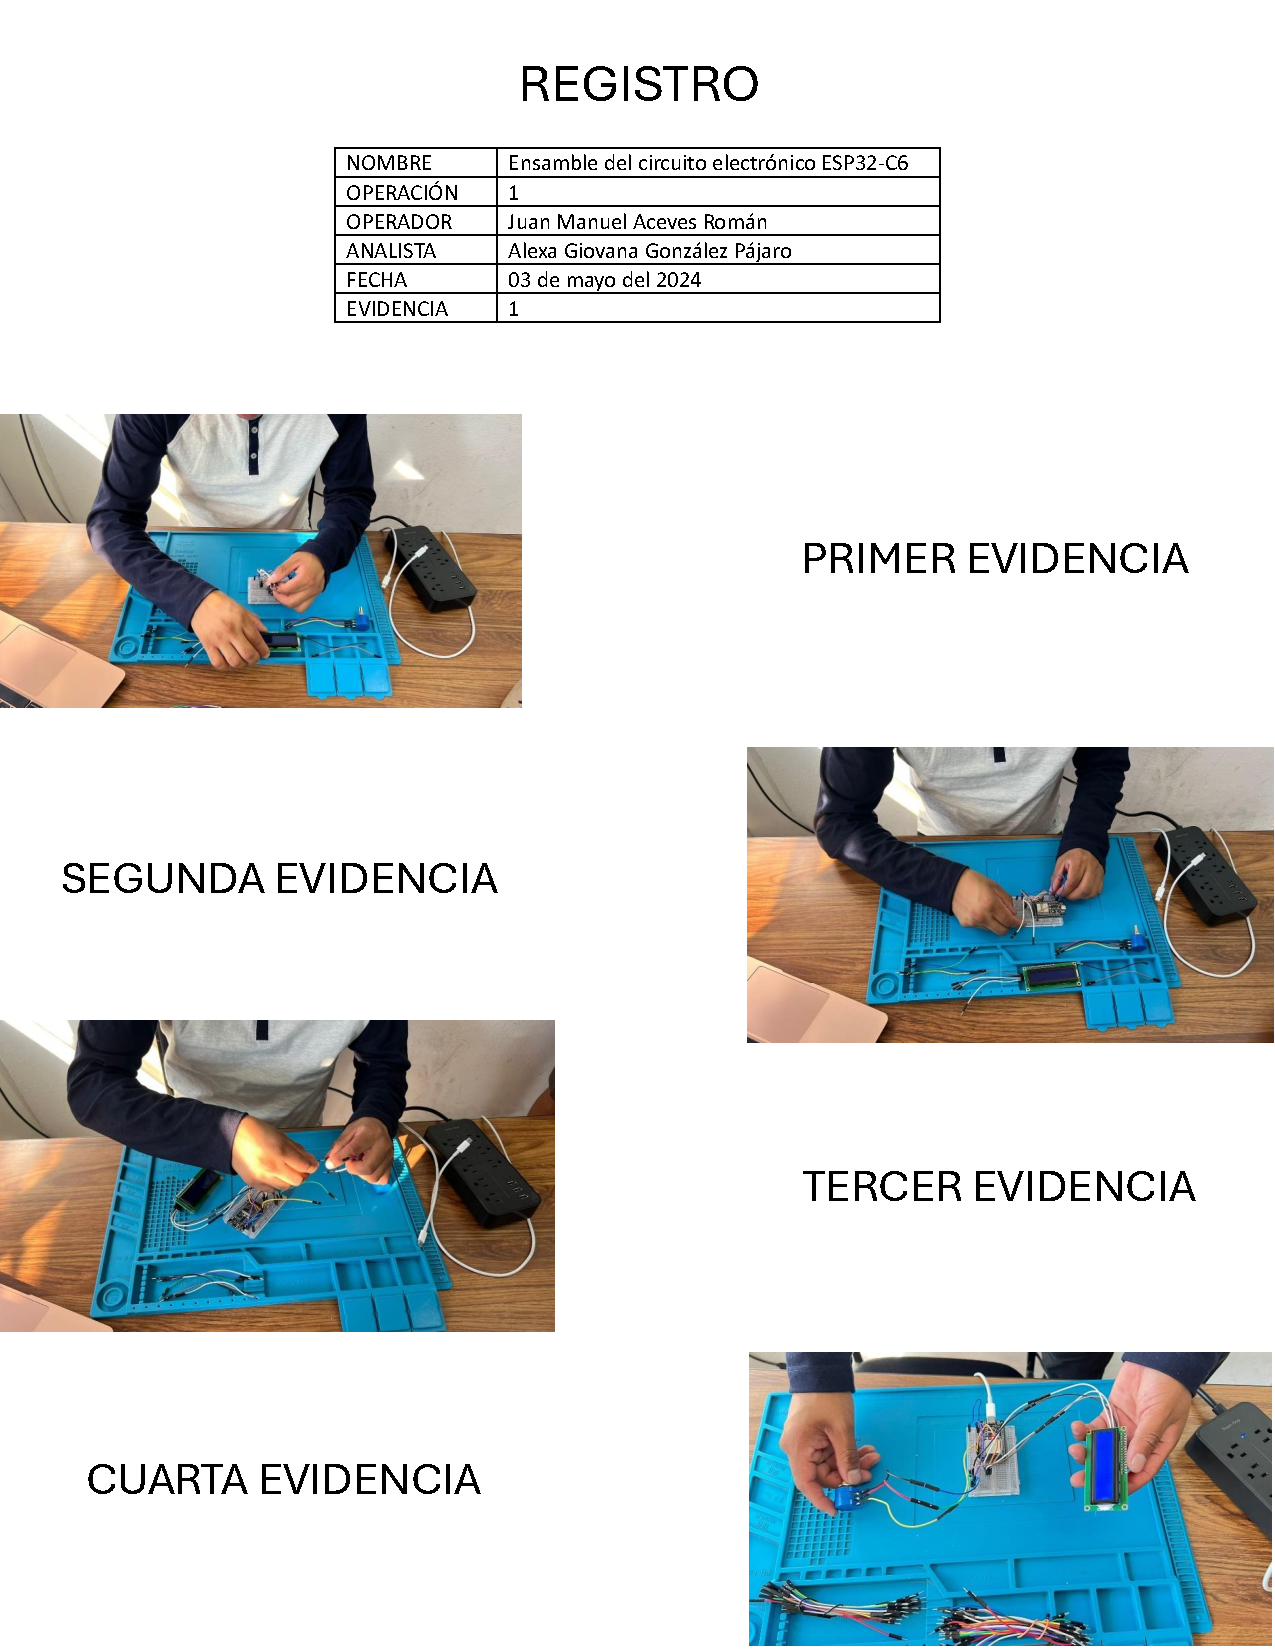
\includepdf[pages=-]{14/img/evidencias.pdf}
    
    %Antes de comenzar a preparar tu artículo, es importante que lea primero la guía del autor, la cual incluye los temas o apartados que son necesarios para tener tu trabajo completo.
    %Una vez completada la edición del texto, el documento está listo para el uso de esta plantilla. En este archivo recién creado, resalte todo el contenido e importe el archivo de texto preparado. Ahora esta listo para estilizar su documento.
    %En esta sección se deben presentar todo lo obtenido de la sección 2, incluidas deducciones o efectos del desarrollo. También se podrán incluir subsecciones numeradas de la siguiente forma:
    
    %\subsection{Autores y Afiliaciones}
    
    Para distinguir las afiliaciones de los autores, utilice superíndices iniciando con el número 1, 2, etc., sucesivamente, esto dependerá de la cantidad de los departamentos a los que estén afiliados los autores. En caso de que todos los autores pertenezcan a una mismo departamento e institución, utilizar sólo el superíndice 1. 
    
    %\subsection{Identificar los encabezados}
    
    Se les recuerda a los autores que los encabezados deben de estar conforme los solicita la guía del autor. De ahí se puede adaptar el trabajo para que sea más fácil de entender para el lector.
    Los encabezados organizan los temas sobre una base relacional y jerárquica. Por ejemplo, el título del documento es encabezado del texto principal porque todo el material posterior se relaciona y elabora sobre este tema. 
    
    %\subsection{Tablas y Figuras}
    
    \begin{enumerate}
        \item Posición de las tablas y figuras: Coloque las figuras y las tablas en la parte superior e inferior de las columnas. Evite colocarlos en medio. Las figuras y las tablas grandes pueden abarcar ambas columnas. Los títulos de las figuras deben de estar debajo de las mismas; los títulos de las tablas deben aparecer encima de ellas. Insértese las figuras y los cuadros después de citarse en el texto. Utilice la abreviatura “Fig. 1”, incluso al principio de una oración. 
    \end{enumerate}
    
    \section{Conclusiones}
    
    Se describe aquí el alcance del trabajo, logros obtenidos y perspectivas para el futuro de este. Se sugiere colocar información cuantitativa obtenida.
    
    \section{Agradecimientos}
    
    Es importante darles su debido reconocimiento a los laboratorios, instituciones, organizaciones, entre otros que han sido participes para la culminación de este trabajo. También es importante mencionar, fondos, proyectos, becas, entre otros que se le han otorgado al o los autores para realizar el trabajo de investigación. Ejemplo: “Los autores agradecen al Concejo Nacional de Ciencia y Tecnología por los recursos otorgados…”
    
    \section*{Referencias}
    
    %Para esta platilla, se solicita al autor enumerar las citas de manera consecutiva entre corchetes \cite{YLi2013}. 
    %La puntuación de la oración que sigues sería \cite{Mesaelides2011}. 
    %Refiérase simplemente al número de referencia, como en \cite{Morales2012}, no utilice “Ref. [3]” o “referencia [3]” excepto al principio de una oración: “La referencia [3] fue la primera…”
    Enumere las notas al pie por separado en superíndices. Coloque la nota de pie de en la parte inferior de la columna en la que se citó. No coloque notas al pie en la lista de referencias. Utilice letras para las notas al pie de la tabla.
    A menos de que haya tres autores o más; no utilice “et al.”. Los trabajos que no hayan sido publicados, incluso si han sido presentados para su publicación, deben ser citados como “inéditos”. Los trabajos que han sido aceptados para su publicación deben de citarse como “en prensa”. Poner en mayúscula sólo la primera palabra de un título, excepto los nombres propios y los símbolos de elemento. 
    %Otros ejemplos \cite{LAAngeles2021}, \cite{LAAngelesConni}. 
    %Véase el link \cite{prueba}, Véase el Apéndice \ref{anexo:pines}.
    
    % Ejemplo
    %  @Article{article,
    % 	author = "Author1 LastName1 and Author2 LastName2 and Author3 LastName3",
    % 	title = "Article Title",
    % 	volume = "30",
    % 	number = "30",
    % 	pages = "10127-10134",
    % 	year = "2013",
    % 	doi = "10.3389/fnins.2013.12345",
    % 	URL = "http://www.frontiersin.org/Journal/10.3389/fnins.2013.12345/abstract",
    % 	journal = "Frontiers in Neuroscience"
    % }
    
    % @book{book,
    %   author    = {Author Name}, 
    %   title     = {The title of the work},
    %   publisher = {The name of the publisher},
    %   address   = {The city},
    %   year      = 1993,
    % }
    
    % @incollection{chapter,
    %   author       = {Bauthor Surname}, 
    %   title        = {The title of the work},
    %   editor       = {Editor Name},
    %   booktitle    = {The title of the book},
    %   publisher    = {The name of the publisher},
    %   address      = {The city},
    %   year         = 2002,
    %   pages        = {201-213},
    % }
    
    % @InProceedings{conference,
    %   author = {Cauthor Name and Dauthor Surname and Fauthor LastName},
    %   title = {The title of the work},
    %   booktitle = {The title of the conference proceedings},
    %   year = 1996,
    %   publisher = {The name of the publisher},
    %   editor = {Editor Name1 and Editor Name2},
    %   pages = {41-50},
    % }
    
    % @book{cho,
    %   author       = {Gauthor Name1}, 
    %   title        = {The title of the work},
    %   publisher = {Country code and patent number},
    %   address      = {Patent Country},
    %   year = 2013
    % }
    
    % @book{patent,
    %   author    = {Hauthor Surname1}, 
    %   title     = {The title of the work},
    %   publisher = {Patent number},
    %   address   = {Patent country},
    %   year      = 2010,
    % }
    
    % % please use misc for datasets
    % @misc{dataset, 
    % 	author = "Author1 LastName1 and Author2 LastName2 and Author3 LastName3",
    % 	title = "Data Title",
    % 	year = "2011",
    % 	doi = "10.000/55555",
    % 	URL = "http://www.frontiersin.org/",
    % }
    
    \bibliographystyle{ieeetr}
    \bibliography{14/referencias}
    % 
    % 
    %%%%%%%%%%%%%%%%%%%%%%%%%%%%%%%%%%
    \appendix
    %%%%%%%%%%%%%%%%%%%%%%%%%%%%%%%%%%
    % 
    % 
    \newpage
    \centering{\section[\appendixautorefname{}]{Apéndice}}\label{anexo:cables}
    \includepdf[pages=-]{14/img/cables de conexión .pdf}
    %
    \centering{\section[\appendixautorefname{}]{Apéndice}}\label{anexo:ESP32-C6}
    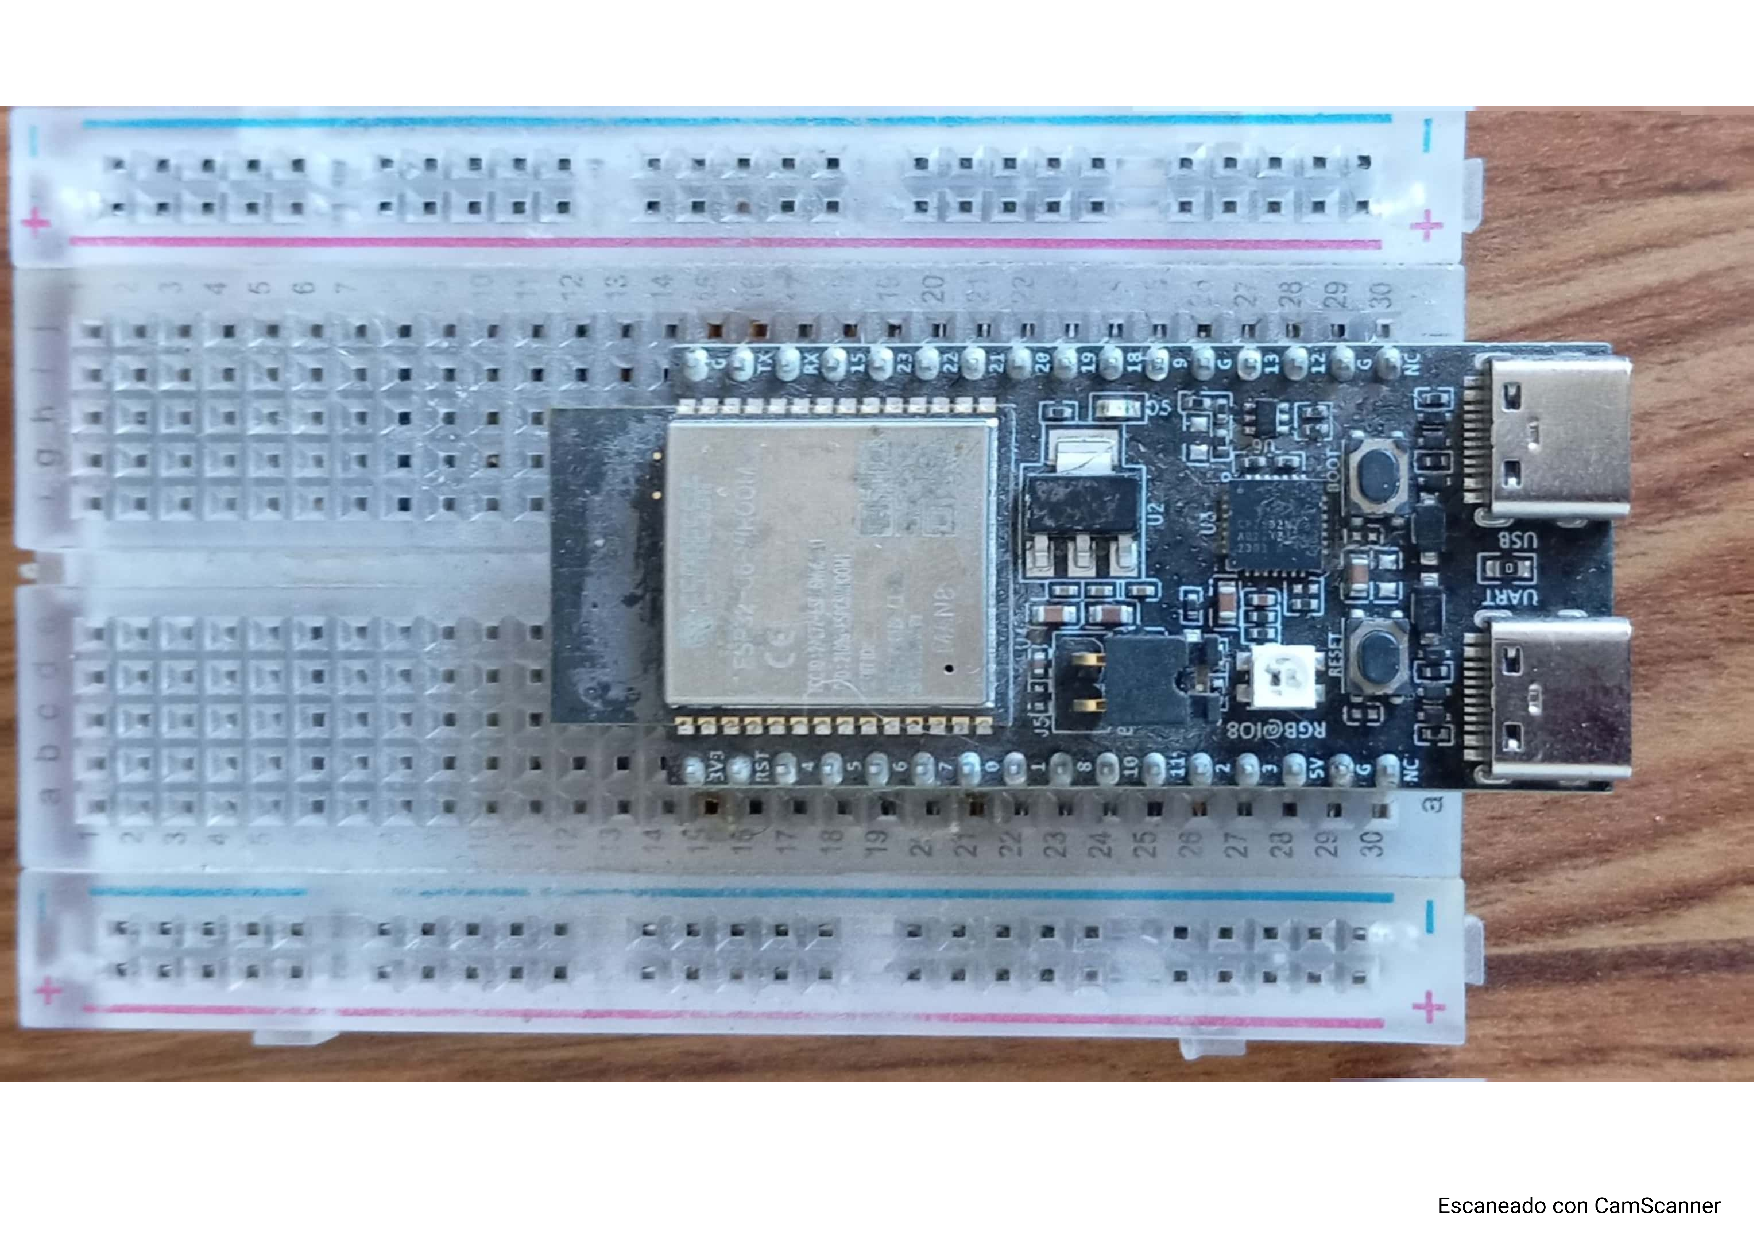
\includepdf[pages=-]{14/img/ESP32-C6.PDF}
    %
    \centering{\section[\appendixautorefname{}]{Apéndice}}\label{anexo:LCD 16x2}
    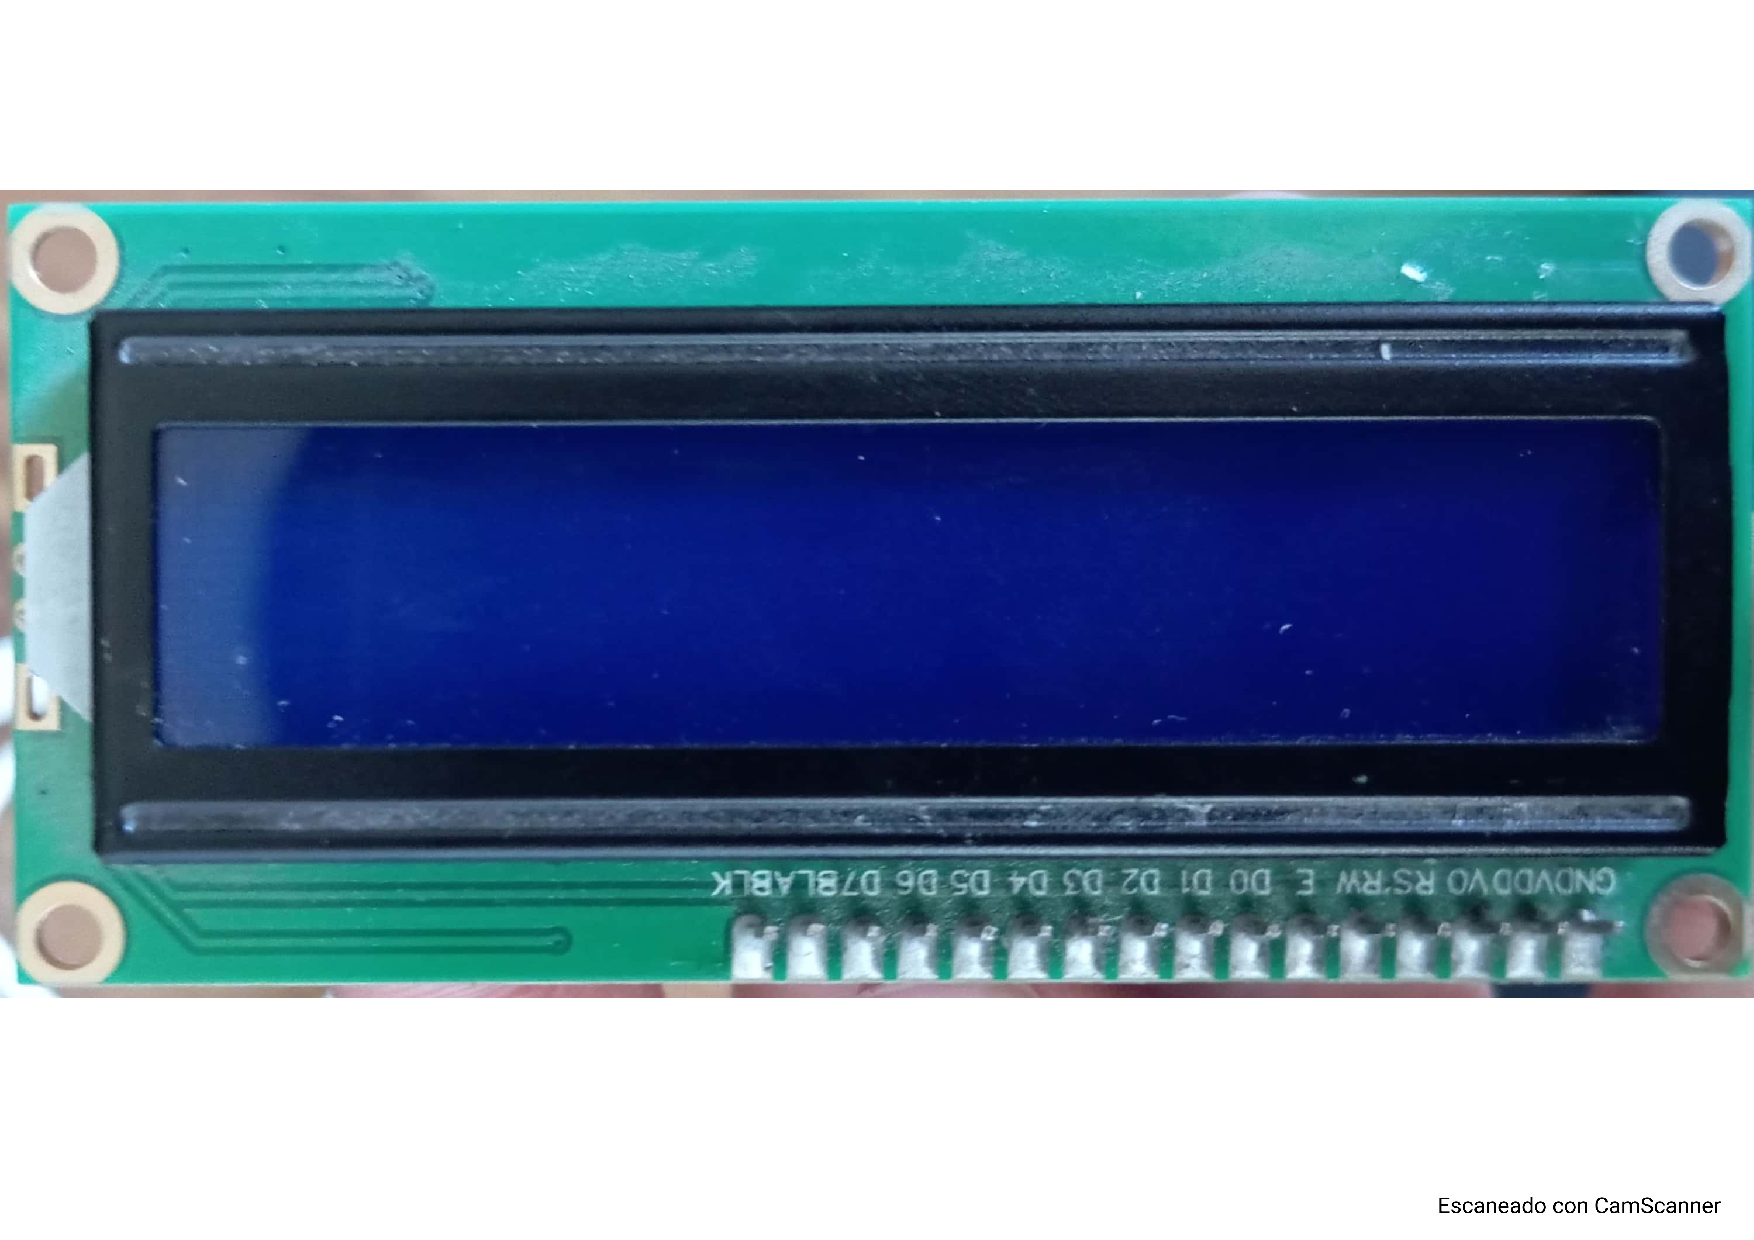
\includepdf[pages=-]{14/img/LCD 16x2.pdf}
    %
    \centering{\section[\appendixautorefname{}]{Apéndice}}\label{anexo:multicontanto}
    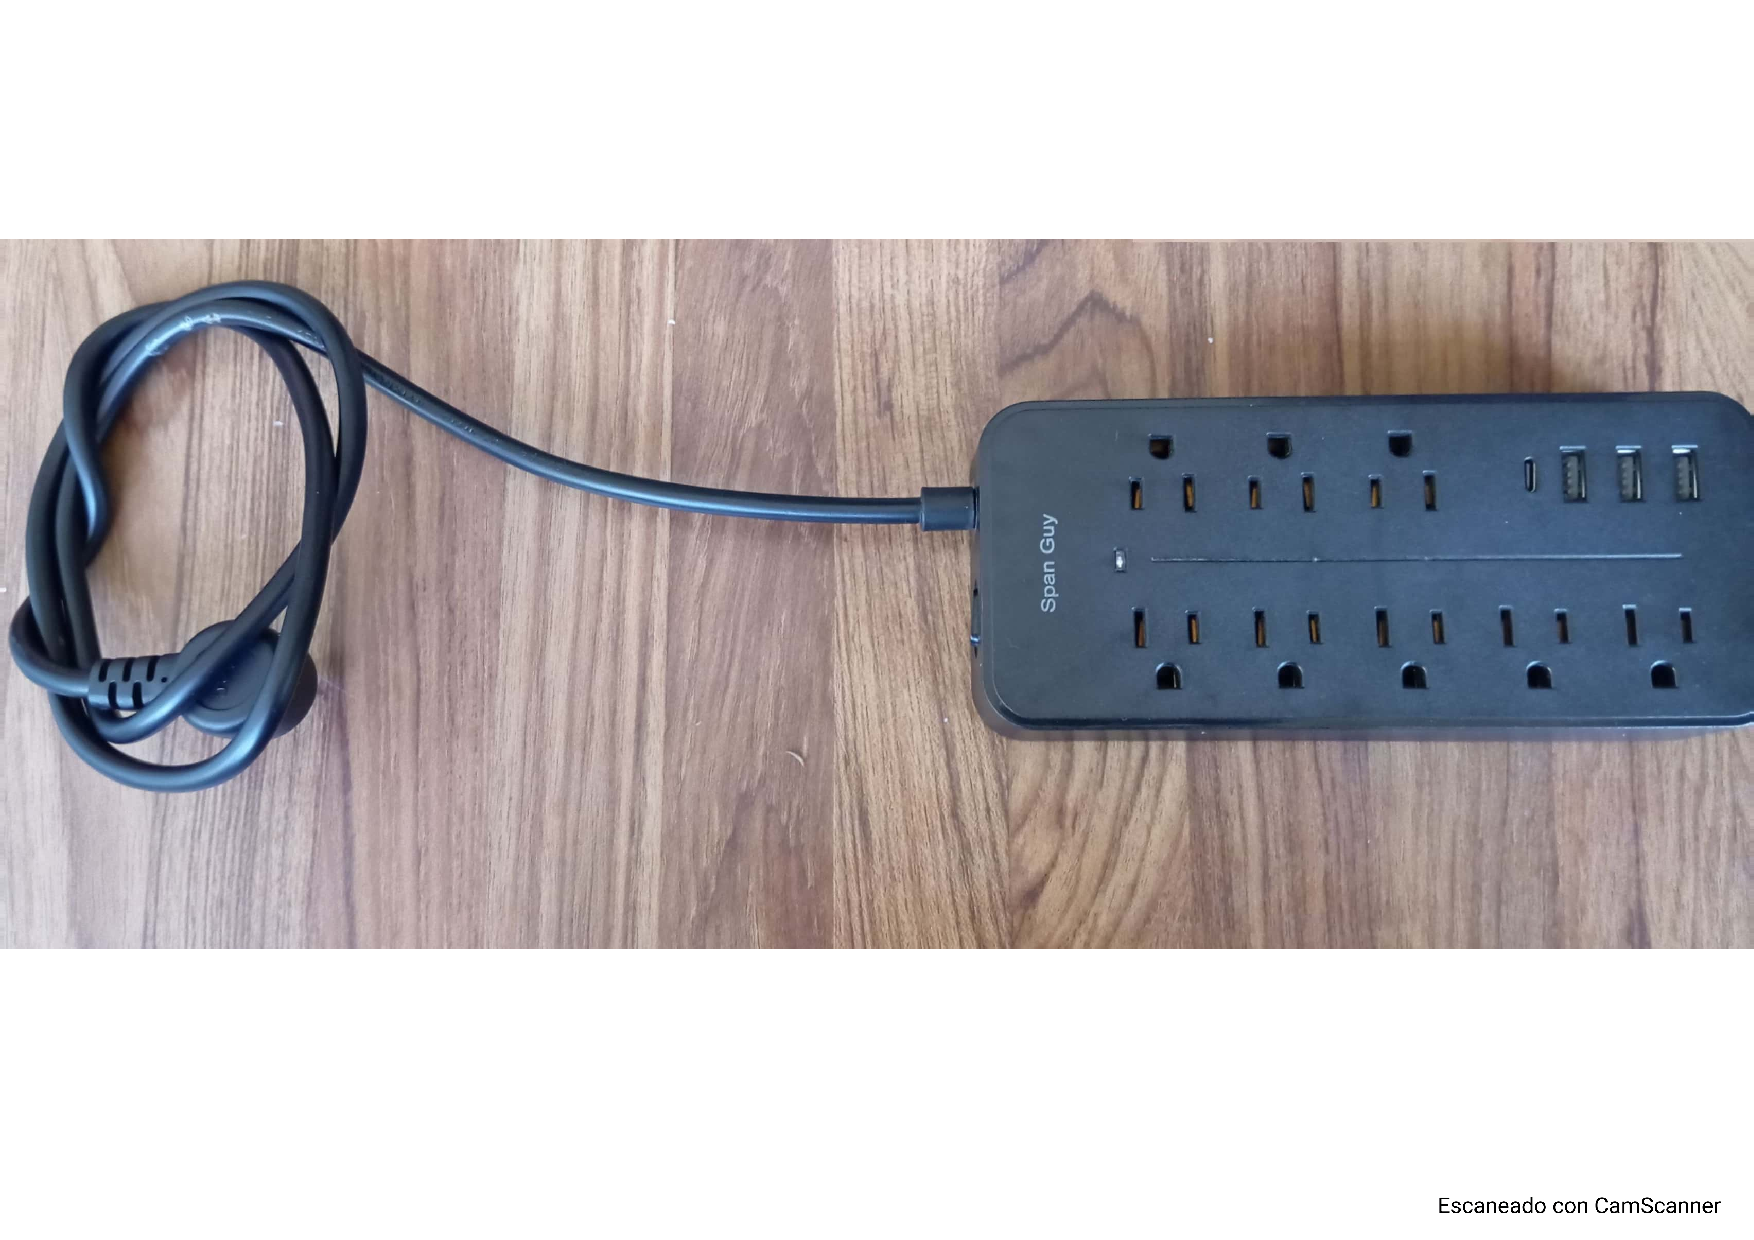
\includepdf[pages=-]{14/img/multicontanto.pdf}
    %
    \centering{\section[\appendixautorefname{}]{Apéndice}}\label{anexo:resistencia}
    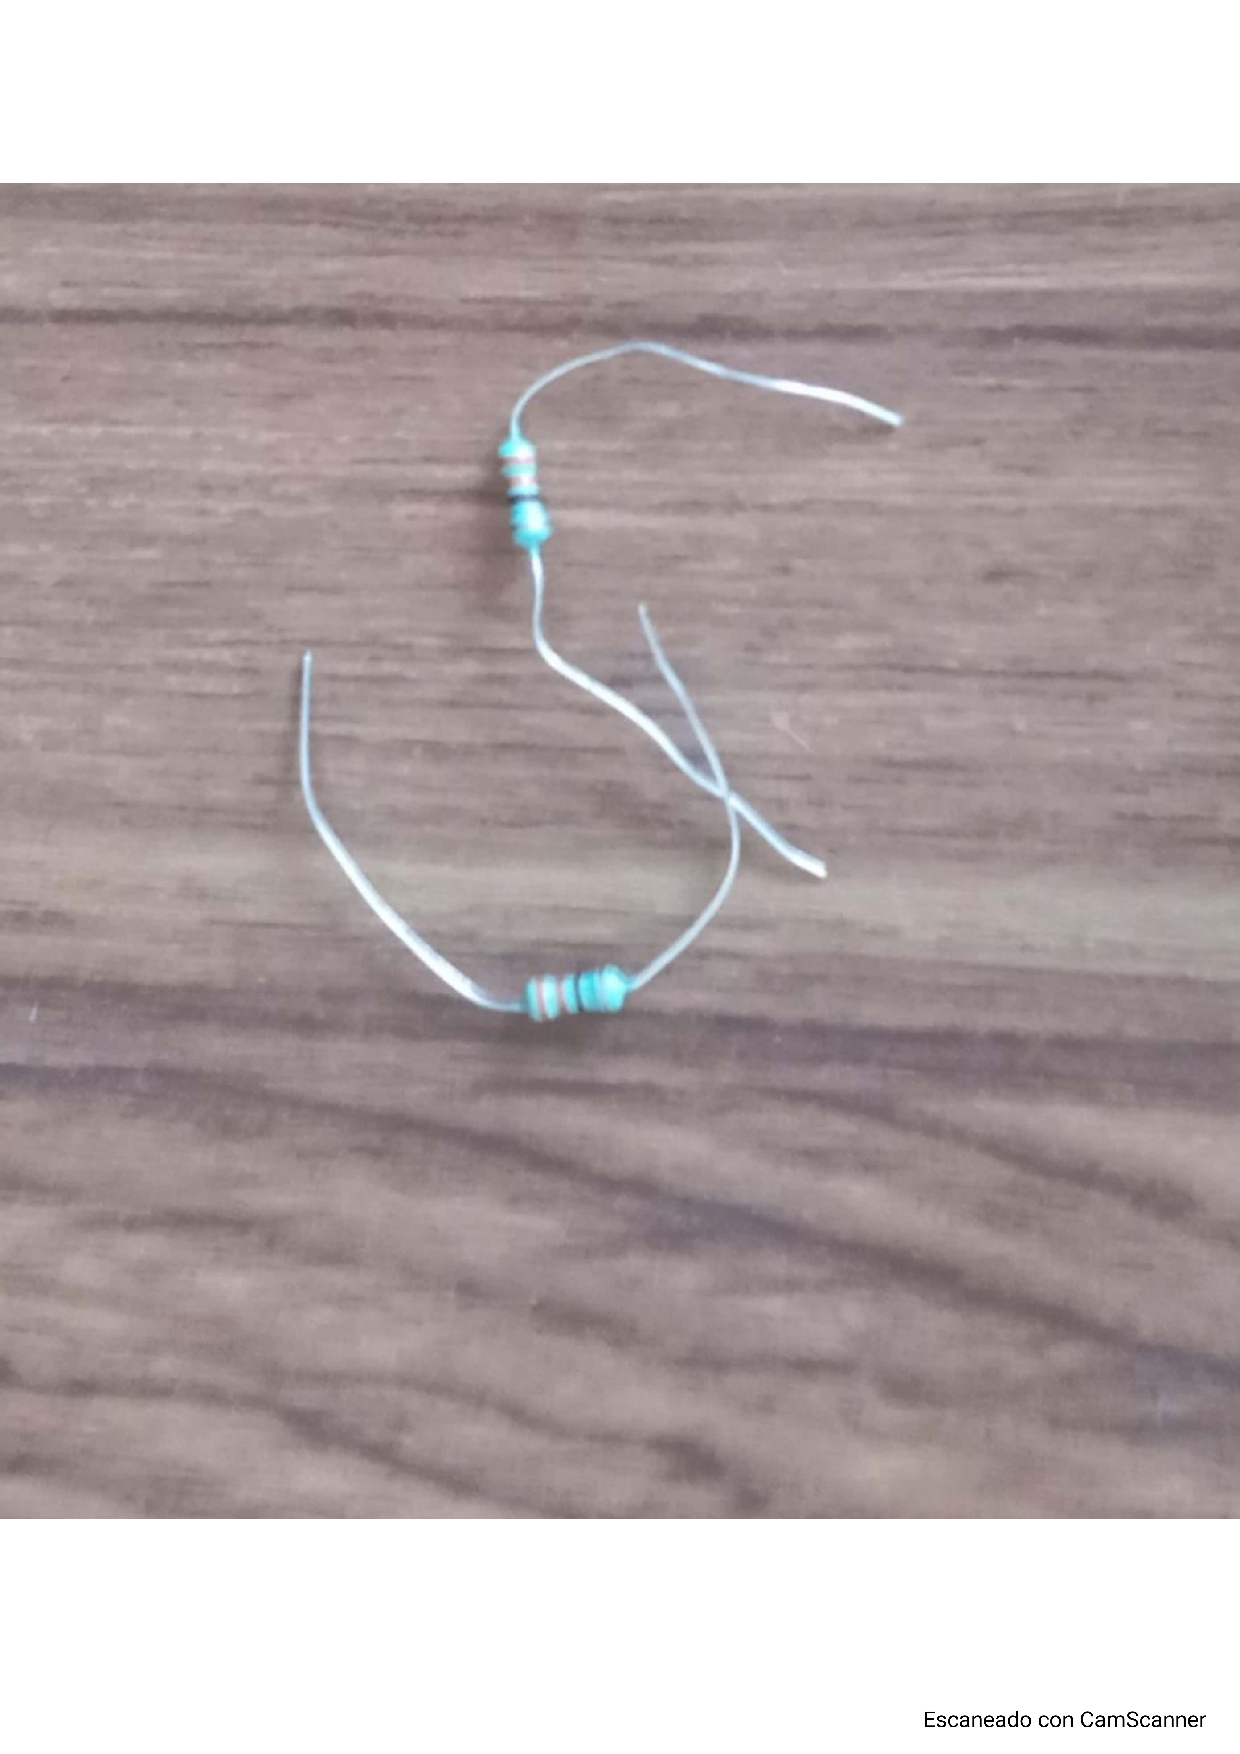
\includepdf[pages=-]{14/img/resistencia.pdf}
    %
    \centering{\section[\appendixautorefname{}]{Apéndice}}\label{anexo:Instructivo}
    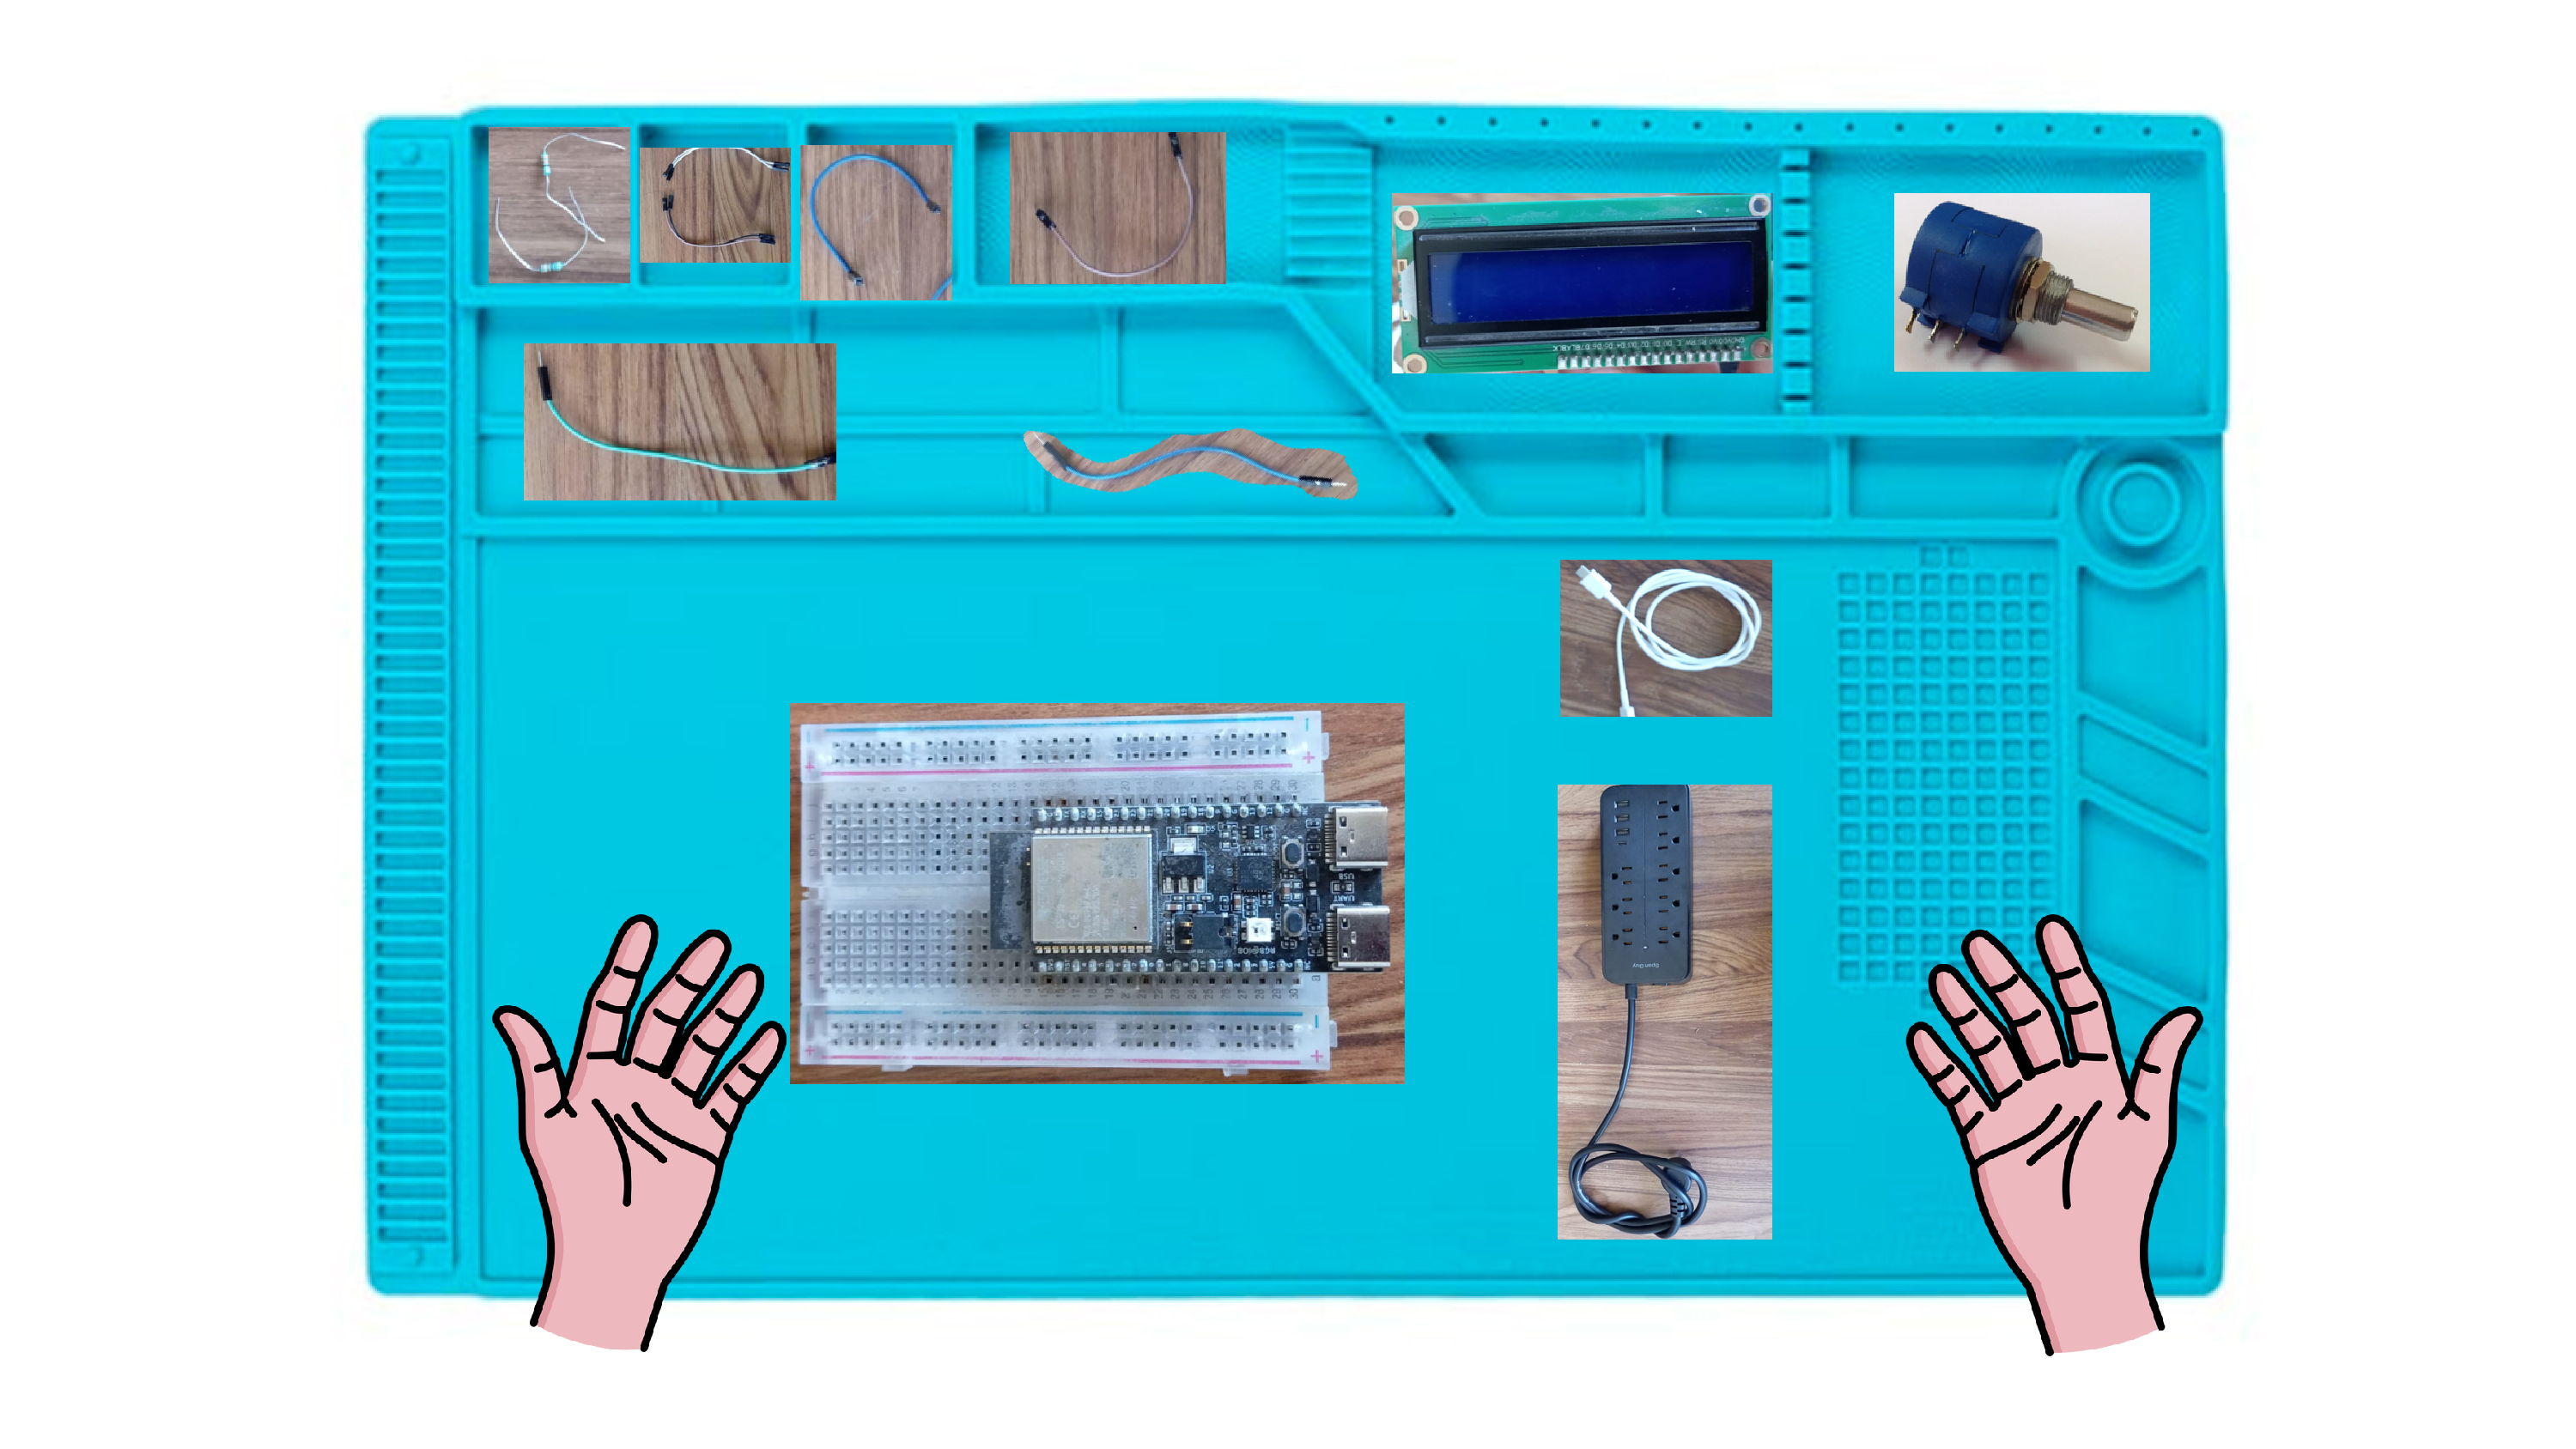
\includepdf[pages=-]{14/img/Instructivo.pdf}
    %
    \centering{\section[\appendixautorefname{}]{Apéndice}}\label{anexo:PlanoCableMh}
    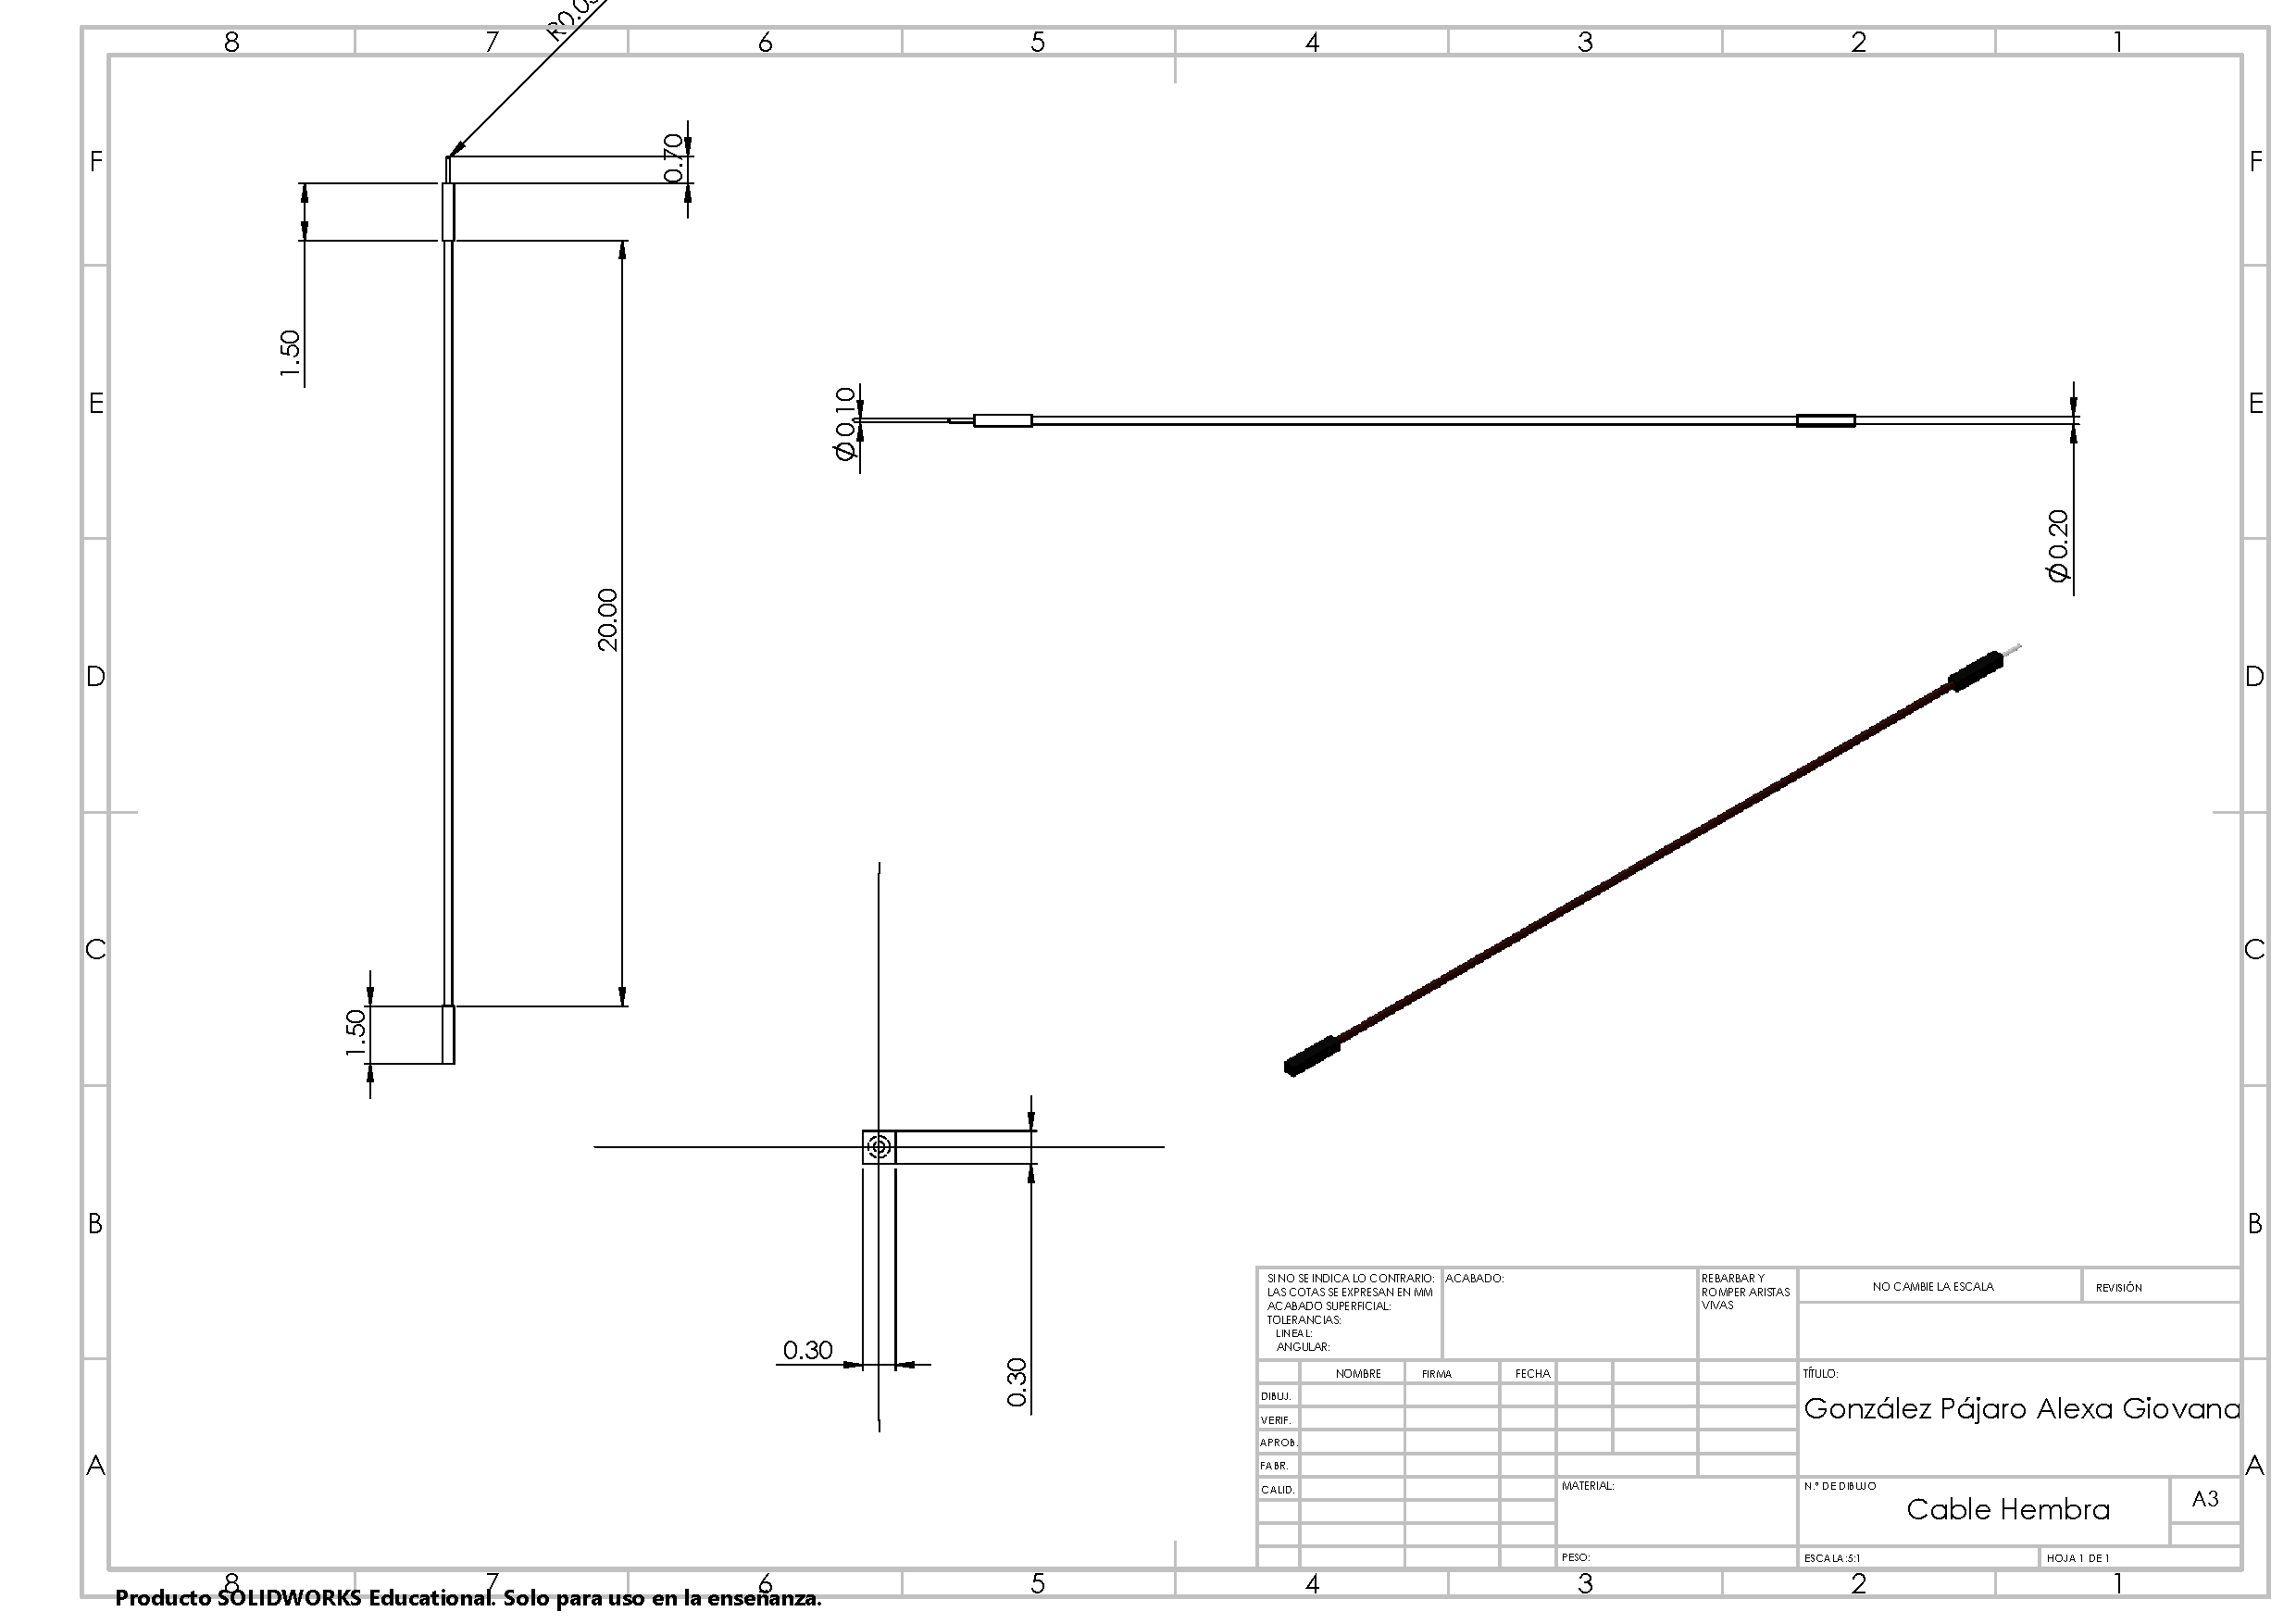
\includepdf[pages=-]{14/img/PlanoCableMh.pdf}
    %
    \centering{\section[\appendixautorefname{}]{Apéndice}}\label{anexo:PlanoCableMm}
    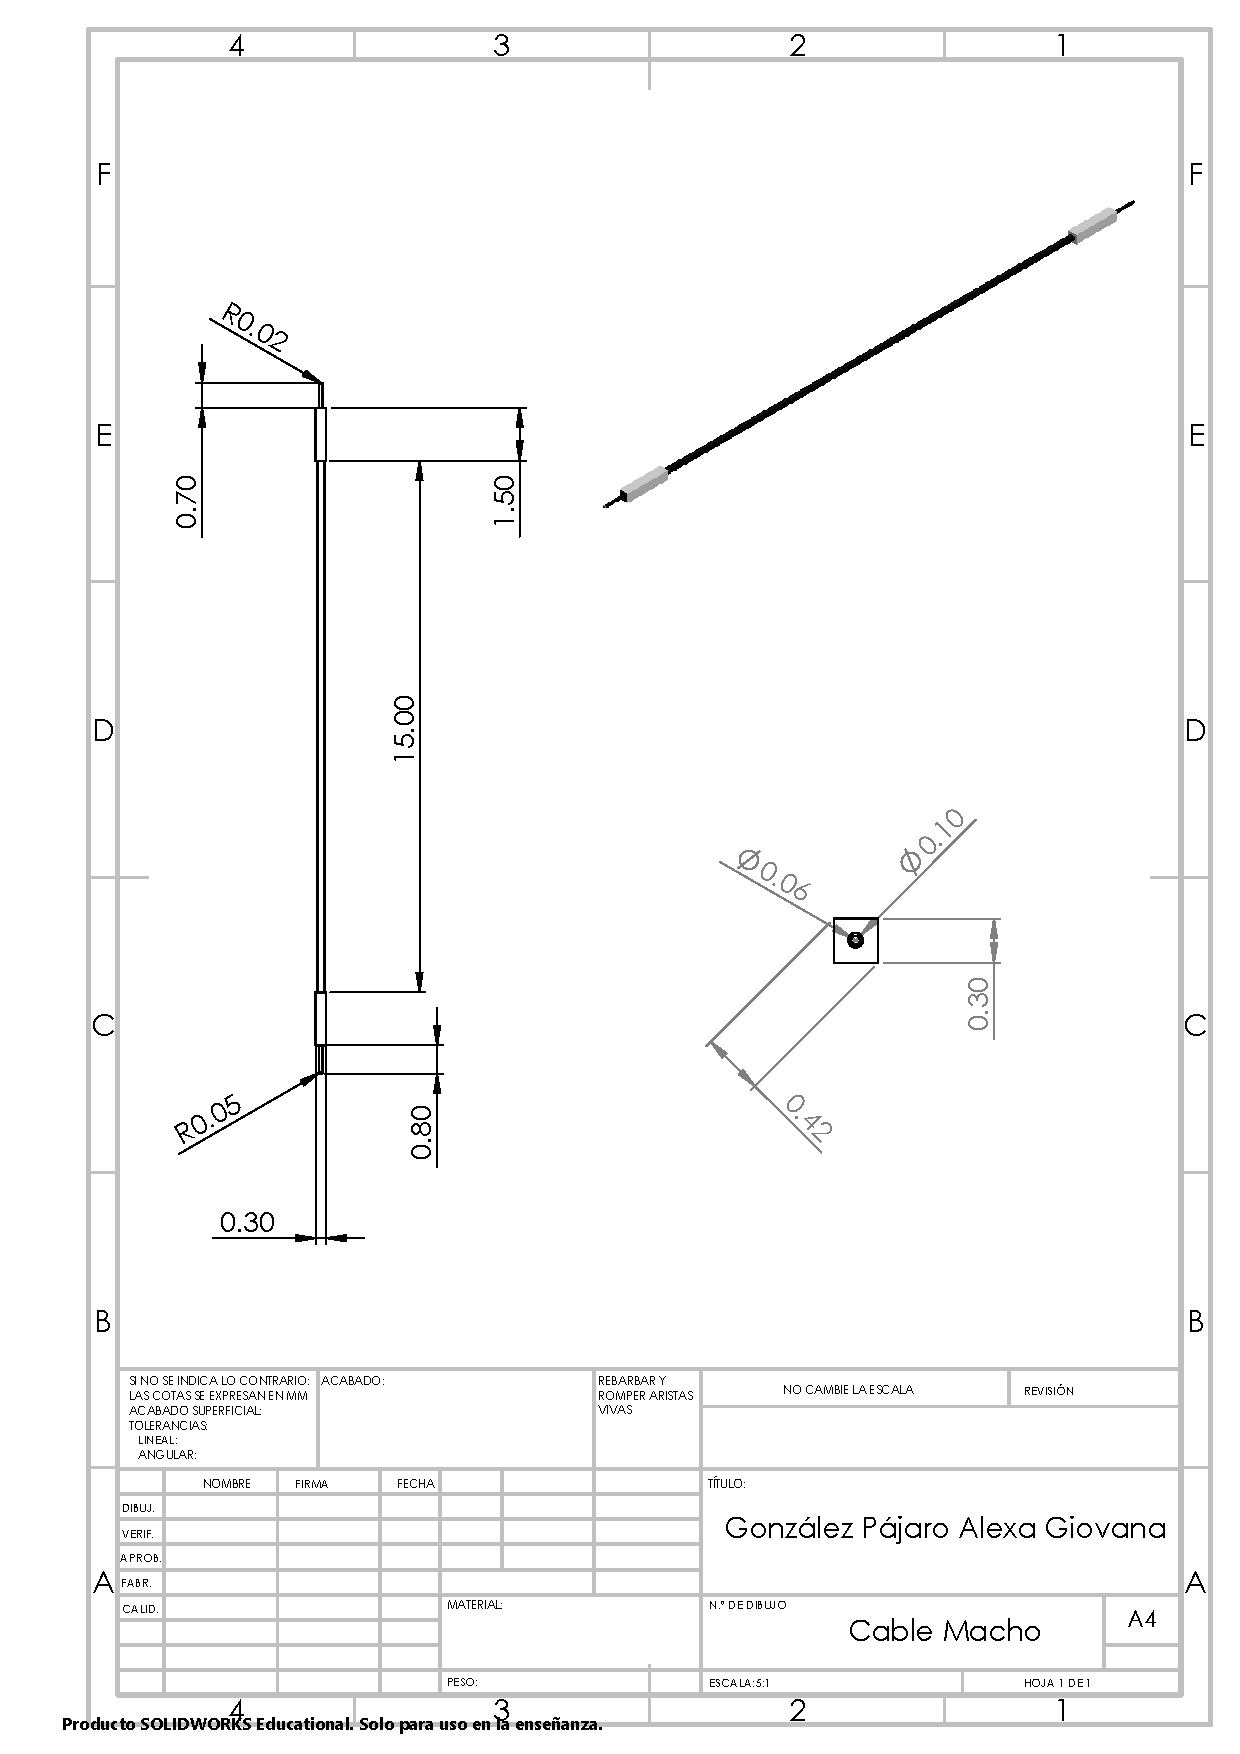
\includepdf[pages=-]{14/img/PlanoCableMm.PDF}
    %
    \centering{\section[\appendixautorefname{}]{Apéndice}}\label{anexo:PlanoLcd}
    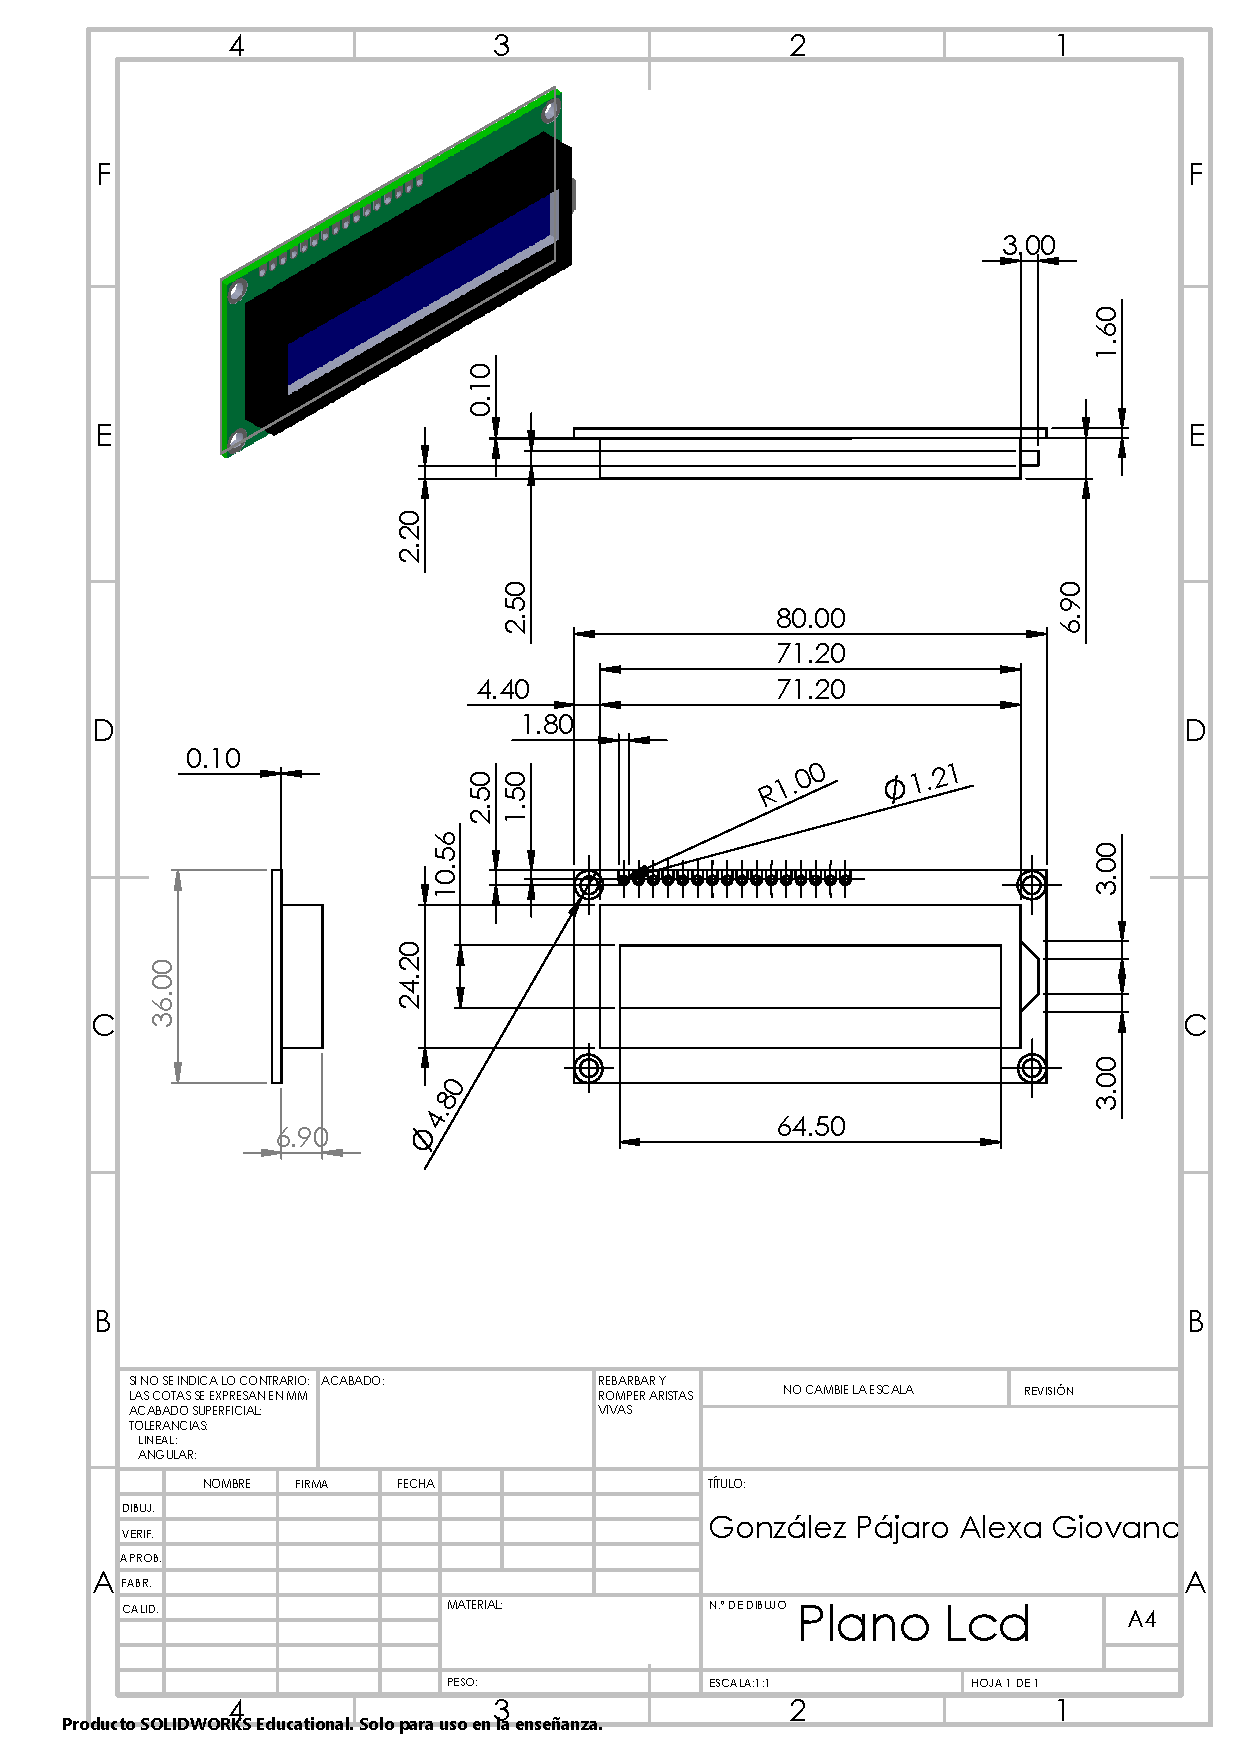
\includepdf[pages=-]{14/img/PlanoLcd.pdf}
    %
    \centering{\section[\appendixautorefname{}]{Apéndice}}\label{anexo:PlanoPotenciometro}
    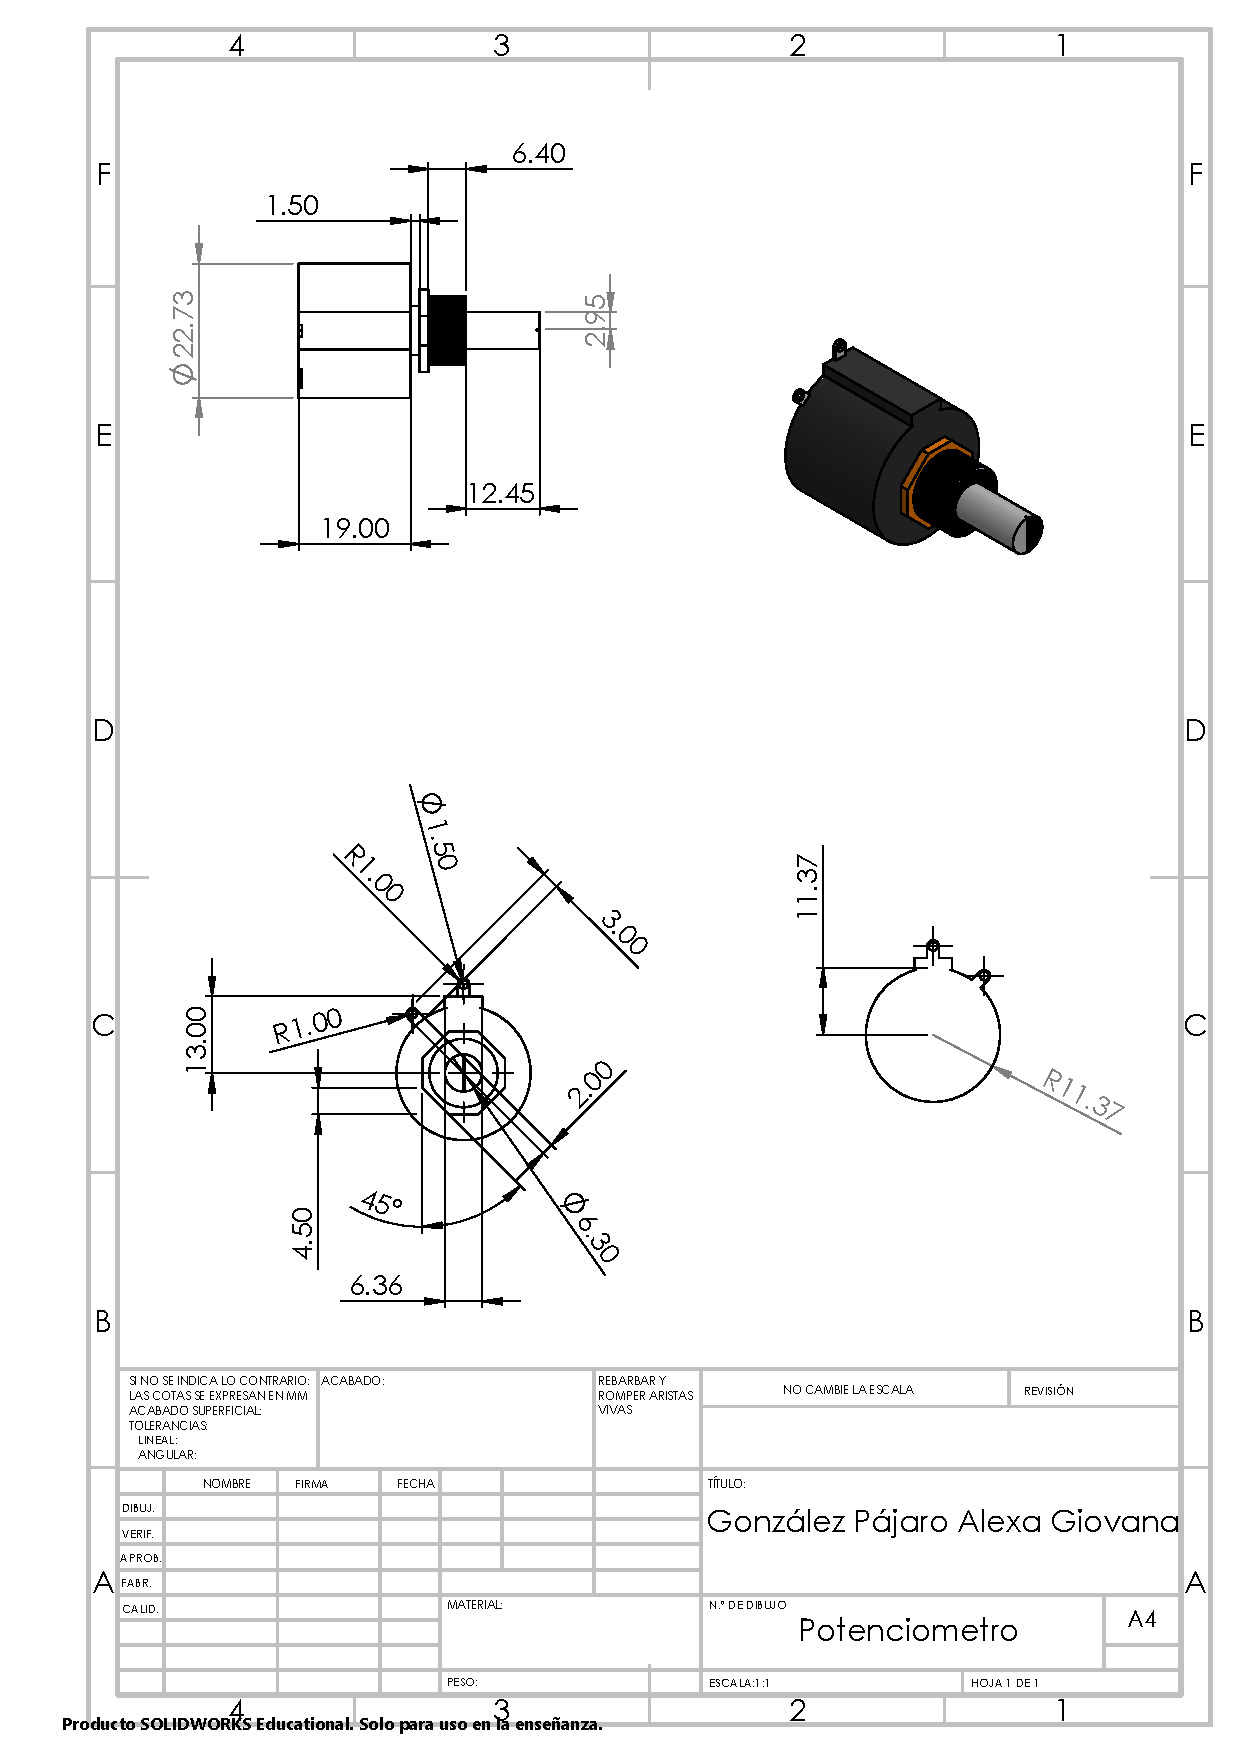
\includepdf[pages=-]{14/img/PlanoPotenciometro.PDF}
    %
    \centering{\section[\appendixautorefname{}]{Apéndice}}\label{anexo:PlanoResistencia}
    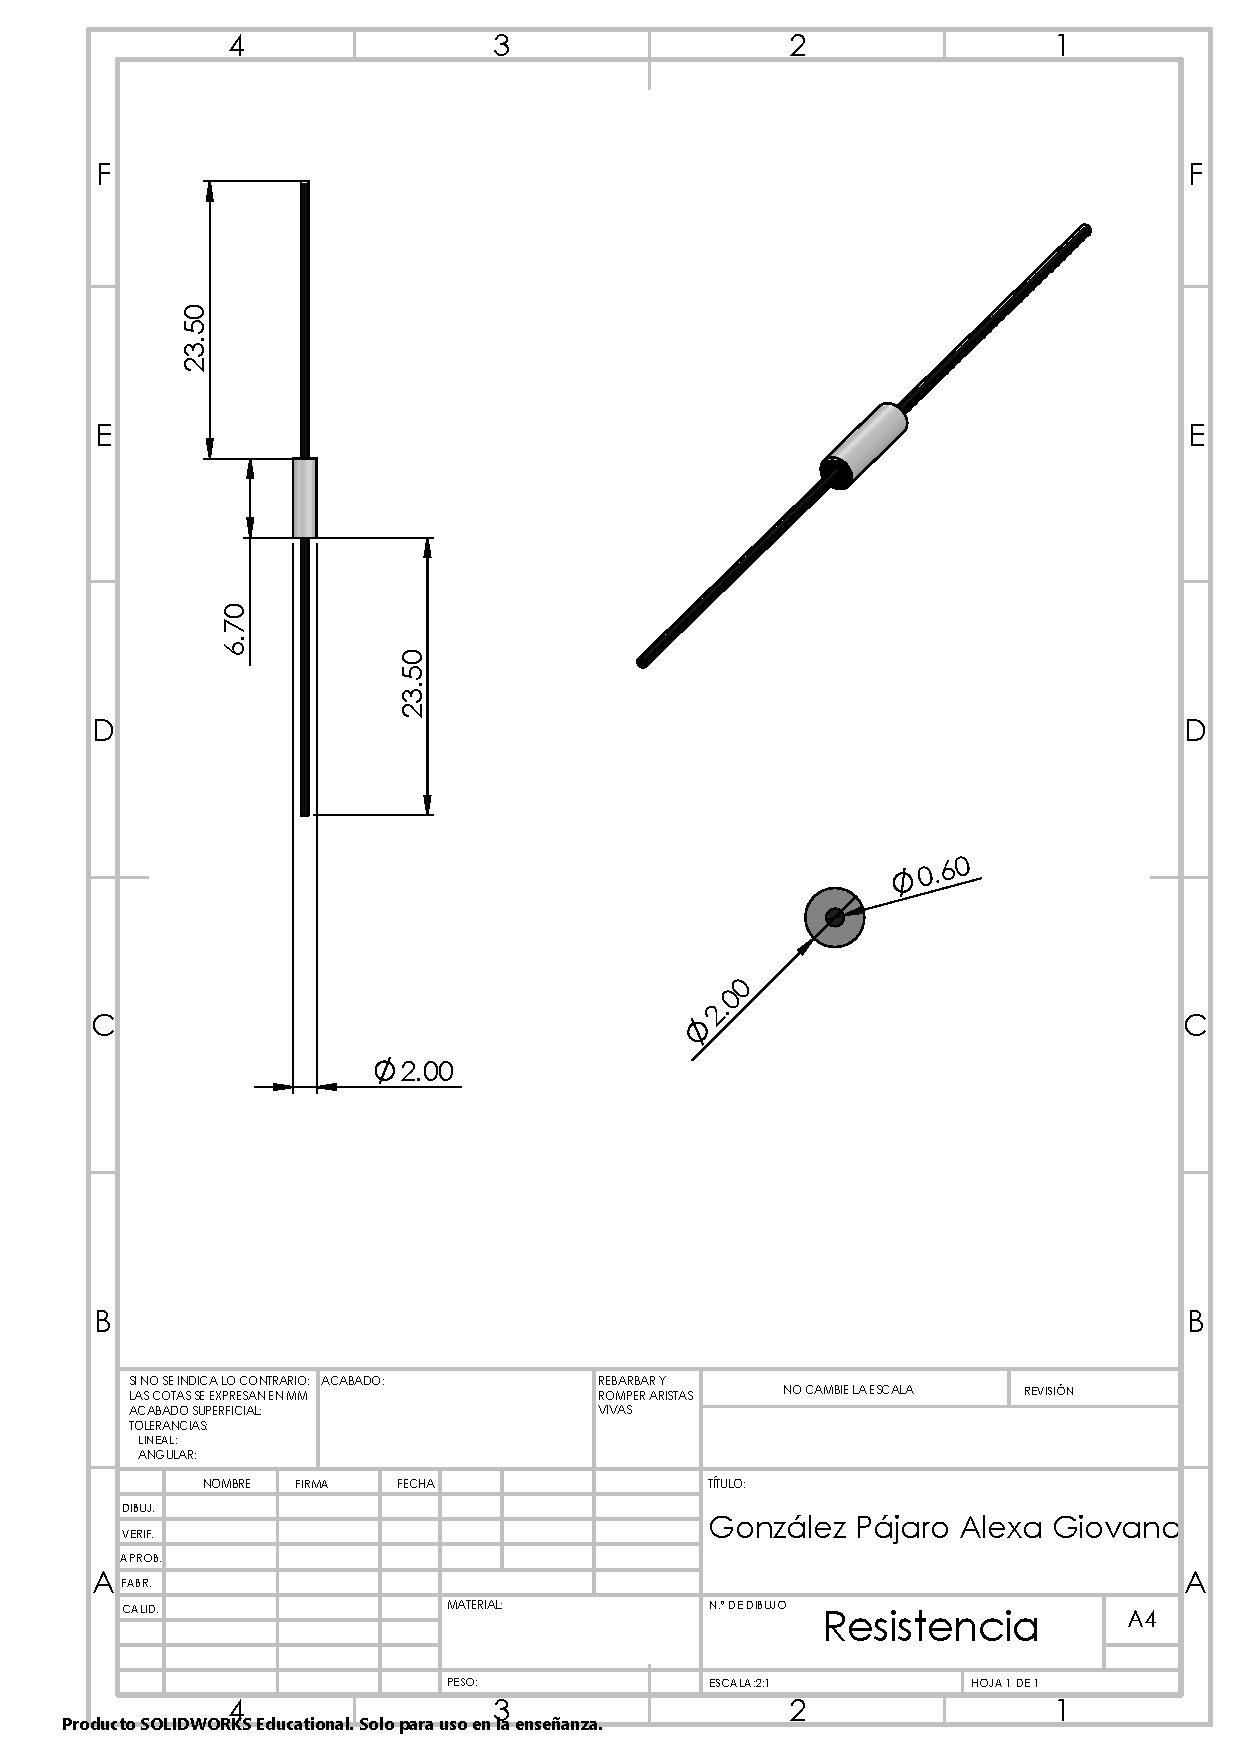
\includepdf[pages=-]{14/img/PlanoResistencia.pdf}
    %%%%%%%%%%%%%%%%%%%%%%%%%%%%%%%%%%%%%%%%